\subsubsection{\textbf{Tree Edit Distance (TREED)}}  

The semantic quality of translated code may depend on its
syntax. Until now, abstract syntax trees(AST) is the most widely-used
structure in representing the syntactic structures in source
code. Therefore, computing the difference of two ASTs is considered as
evaluating syntax difference.  In our study, we apply this idea in
measuring the difference between the syntatic structures of reference
code and translated code. Given a pair of methods in C\# which are
need to be syntactically compared, Roslyn~\cite{tien} is used to parse
them into ASTs. Then, we compute the tree edit distance between two
trees using the algorithm Treed~\cite{oopsla10}.  Specifically, the
tree edit distance is calculated by number of operations
(add,delete,replace,move) to make them identical.

We introduce a formula to normalize the edit distance so that it can
be used in our experiments. The normalized value is computed~as:
\[TREED = 1 -  \frac{TreeEditDistance\left(AST_R, AST_T\right)}{CountNodes \left(AST_R+AST_T\right)}\] 
  
where $TreeEditDistance\left(AST_R, AST_T\right)$ is the editing
distance between two trees $AST_R$ of reference code and $AST_T$ of
translated code; and the denominator is the total number of nodes in
both trees. The value of TREED is from 0 to 1.
%
For any two trees, there will always exist at least one editing (such
as the one that deletes all nodes of the first tree and inserts all
the nodes of the second). Therefore, there will always exist at least
one TREED value and the higher value it is, the more similar those
trees are.

\begin{figure}[h]
	\caption{Tree Editing Example: In the label of each node, its type is in capital font and its val (if exists) is in normal font}
	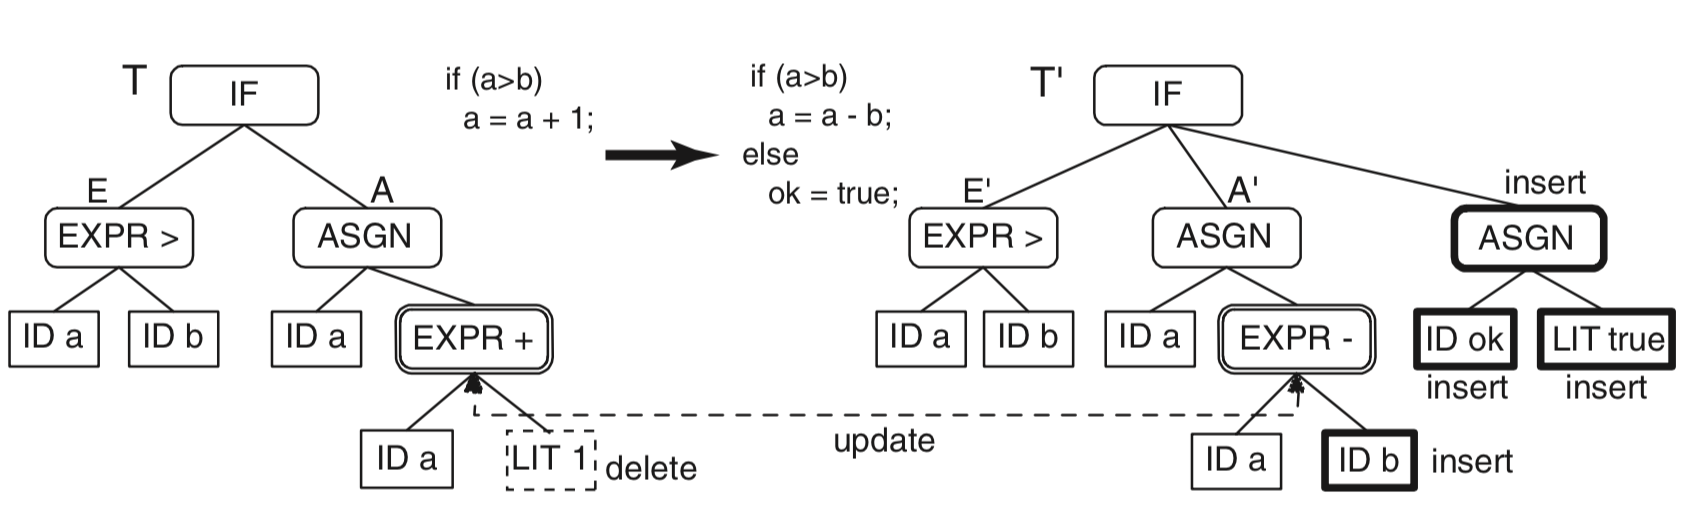
\includegraphics[scale=0.3]{img/treed.png}
	\centering
	\label{fig:treed}
\end{figure}

In the example in Figure \ref{fig:treed}, an \textit{if} statement was
edited by modifying the \textit{if} branch and adding an \textit{else}
branch. The two trees represent the two versions of a method. An edit
consists of one \textit{Delete} (dotted line box), one \textit{Update}
(double-line box), and four \textit{Insert} operations (bold
boxes). Other nodes (single- line boxes) are either unchanged or
moved. Based on the formula of TREED, the result in this case is:
$TREED = 1 - \frac{1 + 1 + 4}{16}=0.625$.



